\documentclass [a4paper, 11pt] {article}

%document configuration
\newcommand{\courseName}{Machine Learning in Graphics \& Vision}
\newcommand{\termYear}{Summer Term 2020}
\newcommand{\homeworkNum}{3}
\newcommand{\studentOne}{Driton Goxhufi}
\newcommand{\studentTwo} {Damir Ravlija}
\newcommand{\matrikelNrStOne}{4233242}
\newcommand{\matrikelNrStTwo}{5503184}
\newcommand{\mailStOne}{driton.goxhufi@student.uni-tuebingen.de}
\newcommand{\mailStTwo}{damir.ravlija@student.uni-tuebingen.de}

%packages
\usepackage [english] {babel}
\usepackage [T1] {fontenc}
\usepackage [utf8] {inputenc}
\usepackage {graphicx}
\usepackage {subcaption}
\usepackage {amsmath}
\usepackage {amssymb}
\usepackage {amstext}
\usepackage {amsthm}
\usepackage {listings}
\usepackage {tikz}

% '{ }' added to force space after the command
\usepackage[
pdftex,
pdfauthor={Goxhufi, Driton; Ravlija, Damir},
pdftitle={MLGV - Exercise \homeworkNum { }Submission},
pdfsubject={Machine Learning in Graphics \& Vision Homework}
]{hyperref}

\usepackage[a4paper,lmargin={2cm},rmargin={2cm},tmargin={3.5cm},bmargin = {2.5cm},headheight = {4cm}]{geometry}

\usepackage[shortlabels]{enumitem}
\usepackage{lastpage}
\usepackage{fancyhdr}

\usepackage{lipsum}
\usepackage{ifthen}

\pagestyle{fancy}



%other config
\renewcommand{\v}[1]{\boldsymbol{#1}}
\newcommand{\mat}[1]{\boldsymbol{#1}}
\newcommand{\m}[1]{\begin{pmatrix}#1\end{pmatrix}}
\newcommand{\tr}[2]{{}^{#1}T_{#2}}
\graphicspath{{./images/}}


\lhead{\begin{tabular}{l}
		\courseName\\
		\termYear \\
		Exercise \homeworkNum
\end{tabular}}
\rhead{\begin{tabular}{lr}
		\studentOne & \matrikelNrStOne \\
		\studentTwo & \matrikelNrStTwo \\
\end{tabular}}

\begin{document}
	
\title{\vspace{-1.5cm}\textbf{Exercise \homeworkNum} \\ 
	\courseName}
\author{\begin{tabular}{lcr}
		\studentOne & \matrikelNrStOne & \href{mailto:\mailStOne}{\mailStOne} \\
		\studentTwo & \matrikelNrStTwo & \href{mailto:\mailStTwo}{\mailStTwo} 
\end{tabular}}	
\date{}
\maketitle


\section{Task 1}
\begin{enumerate}
\item[(a)]
After 15 epochs our model achieves $98.92$ validation accuracy \ref{fig:1}.
State-of-the-art accuracy on classifying MNIST digits reported in the literature is $	99.84$ \footnote{https://paperswithcode.com/sota/image-classification-on-mnist}.

\begin{figure}[!h]
	\centering
	\begin{subfigure}{0.7\textwidth}
		\centering
		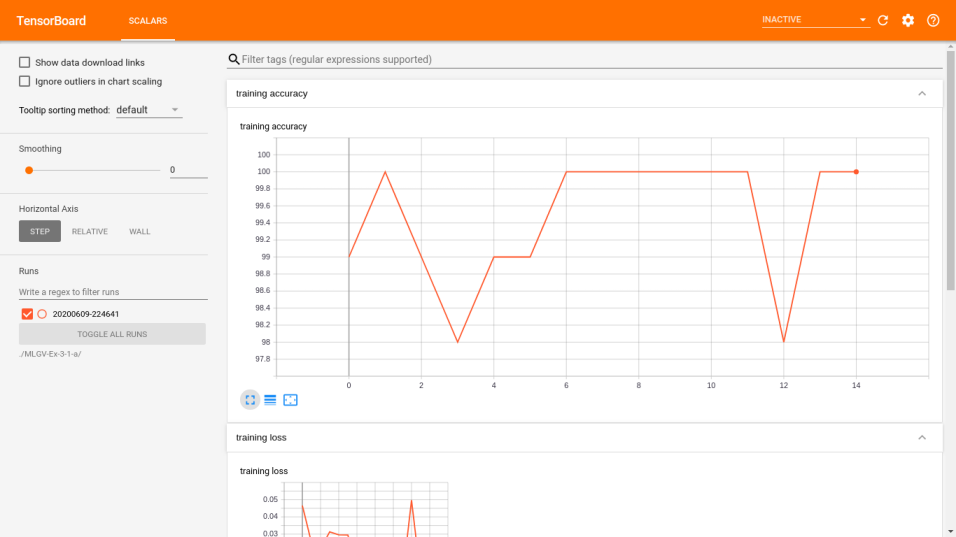
\includegraphics[width=\textwidth]{img/3-1-a-train-epoch.png}
		\caption{Training accuracy against the epochs}
		\label{fig:2a}
	\end{subfigure}
	\begin{subfigure}{0.7\textwidth}
		\centering
		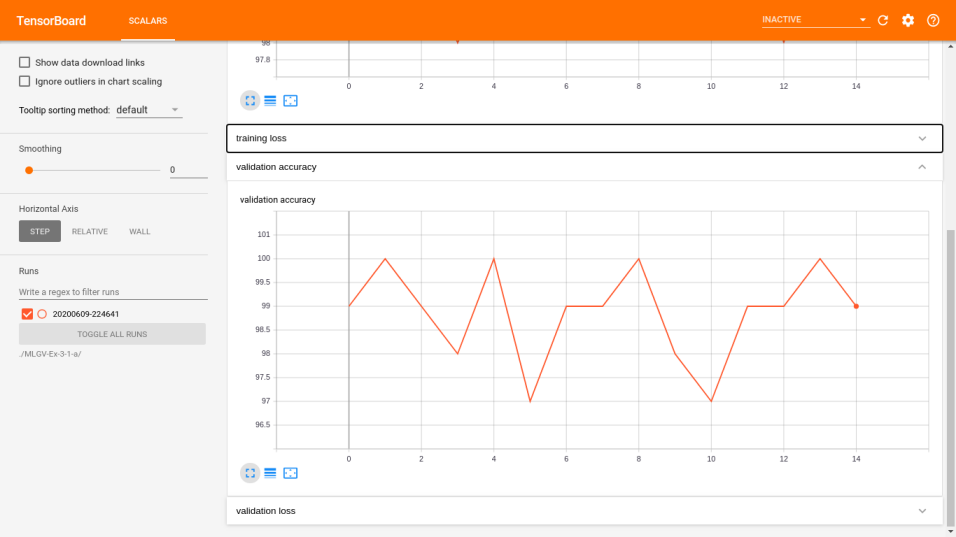
\includegraphics[width=\textwidth]{img/3-1-a-valid-epoch.png}
		\caption{Validation accuracy against the epochs}
		\label{fig:2b}
	\end{subfigure}
	\caption{Plot of results from task 3.1.(a)}
	\label{fig:1}
\end{figure}

\item[(b)]
Model summary is shown in Figure \ref{fig:2}. Output shape of \texttt{torch.nn.conv2d} with zero padding for an input of shape $[B, T, T, C]$ and stride 2 kernel-size 3 can be computed in the following way (under the assumption that $B$ is batch size, first $T$ is the number of channels, second $T$ is the input height and $C$ is the input width):
\begin{itemize}
	\item Batch size $B$ stays the same.
	\item As the kernel-size is larger than 2 and there are zero padding, both height and width have to decrease and since the stride 2 is also used, the resulting height is ceil$(\frac{T}{2})$ and the resulting width is floor$(\frac{C}{2})$.
	\item The resulting output shape: $[B, T, \text{ceil}(\frac{T}{2}), \text{ceil}(\frac{T}{2})]$ if we assume that the number of output channels is the same as the number of input channels $T$.
\end{itemize}
	

\begin{figure}[!h]
	\centering
	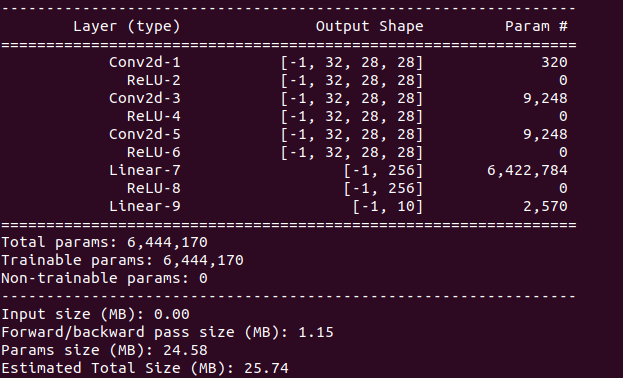
\includegraphics[width=0.8\textwidth]{img/3-1-b.png}
	\caption{Model summary obtained using \texttt{torchsummary} package task 3.1.(b)}
	\label{fig:2}
\end{figure}


\item[(c)]
After training 15 epochs we get $92.07$ validation accuracy. 
We tested our model with different learning rates, but in the end settled on the value of $0.001$ as it seemed that the lower learning rate doesn't improve accuracy, but only increases training rate. To increase training speed we included batch normalization layers. 
\end{enumerate}


	
\end{document}

